\documentclass{beamer}
% Load csquotes for the \enquote command
\usepackage{csquotes}
\usepackage{hyperref}
% Load biblatex for bibliography management
\usepackage[backend=biber, style=authoryear]{biblatex}
\addbibresource{bibliography.bib} % Specify your BibTeX bibliography file

\mode<presentation> {
\usetheme{CambridgeUS}
\usecolortheme{seahorse}
}

\title{Macroéconomie 1}
\author{Mart\'in Valdez}
\date{IE1}

\begin{document}

\begin{frame}
\titlepage
\end{frame}

% \begin{frame}
% \frametitle{Overview}
% \tableofcontents
% \end{frame}

% ------------------------------------------------
%  Introduction
% ------------------------------------------------

\section{Introduction}
\begin{frame}
    \frametitle{Introduction}
    \begin{itemize}
        \item Aperçu du cours
        \begin{itemize}
            \item Introduction à la macroéconomie
            \item Concepts, modèles et données macroéconomiques
            \item Croissance économique
            \item Consommation
            \item (Peut-être) Modèle de croissance néoclassique
        \end{itemize}
        \item Objectifs : Découvrir la macroéconomie, peut-être que cela vous plaira !
        \item Évaluation : À discuter.
    \end{itemize}
\end{frame}
%------------------------------------------------
%  Economic Concepts
%------------------------------------------------
\section{Economic Concepts}
\begin{frame}
\frametitle{Micro vs. Macro}
\begin{itemize}
    \item \textbf{Microéconomie:}
    L'étude des agents économiques individuels tels que les ménages et les entreprises,
    comment ils prennent des décisions, et comment ils interagissent dans les marchés individuels.
    \pause
    \item \textbf{Macroéconomie}
    L'étude de l'économie dans son ensemble, incluant des mesures globales telles que
    le PIB, la consommation, l'investissement, l'inflation et le chômage.
    \begin{itemize}
        \item \textbf{Short-run (Court terme):} Cycles économiques, récessions, et politiques monétaires et fiscales.\pause
        \item \textbf{Long-run (Long terme) :} Croissance économique, productivité et commerce international.
    \end{itemize}
\end{itemize}
\end{frame}

\begin{frame}
    \frametitle{Micro vs. Macro}
    \textbf{Pourquoi étudier la macroéconomie ?}
    \begin{itemize}\pause
        \item \textbf{C'est important :} 
        La macroéconomie a un impact direct sur la vie des gens.\pause
        \item \textbf{C'est utile :} Politiciens ont en besoin pour 
        prendre des décisions éclairées sur les politiques économiques.\pause
        \item \textbf{Responsabilité sociale :} Comprendre les politiques économiques.
    \end{itemize}
    \end{frame}
    
    

%------------------------------------------------
%  History of Macroeconomics
%------------------------------------------------
\section{History of Macroeconomics}
\begin{frame}
    \frametitle{Histoire de la Macroéconomie}
    \framesubtitle{Pré-critique de Lucas : 1936-1976}
        \begin{itemize}
            \item Le livre fondateur de John Maynard Keynes en 1936, 
            \enquote{Théorie générale de l'emploi, de l'intérêt et de la monnaie}.
            \item \textbf{Économie keynésienne :} Prône l'intervention gouvernementale 
            pour stabiliser l'économie.
            \item \textbf{Limitations :} 
            Basée sur des relations agrégées telles que la courbe de Phillips,
            une relation inverse entre l'inflation et le chômage \parencite{Phillips_1958}.
            \item Échec dans les années 1970 en raison de la stagflation, une combinaison d'inflation élevée et de chômage élevé,
            qui n'était pas expliquée par les modèles keynésiens.
        \end{itemize}
    \end{frame}
    \begin{frame}
        \frametitle{Histoire de la Macroéconomie}
        \framesubtitle{Post-critique de Lucas : 1976-Présent}
                \begin{itemize}
                    \item \textbf{La critique de Robert Lucas en 1976 :} Les micro-fondations sont essentielles pour les modèles macroéconomiques ! \parencite{Lucas_1976}.
                    \item A conduit au développement de la macroéconomie moderne, à commencer par la théorie du cycle économique réel \textcite{Kydland_Prescott_1982}.
                    \item \textbf{Principales réflexions :} Les attentes, la rationalité et les chocs.
                    \item \textbf{Économie néo-keynésienne :} Intègre les prix et les salaires rigides dans les modèles : modèles \textbf{DSGE}.
                \end{itemize}
    \end{frame}
                        
%------------------------------------------------
%  Economic Models
%------------------------------------------------
\begin{frame}
    \frametitle{Modèles Économiques}
    \framesubtitle{Introduction}
    Qu'est-ce qu'un Modèle ?
    \pause
        \begin{itemize}
            \item Un modèle est une \textbf{représentation simplifiée} d'une réalité complexe.
            \item Les modèles nous aident à comprendre, expliquer et prédire les phénomènes économiques avec un cadre clair.
            \item \textbf{Objectif :} Abstraire le monde réel complexe en parties gérables.
        \end{itemize}
    \end{frame}
    \begin{frame}
        \frametitle{Modèles Économiques}
        \framesubtitle{Introduction}
        Pourquoi les modèles sont-ils importants ?
        \pause
        \begin{itemize}
            \item \textbf{Réalisation d'expériences:} Les modèles permettent aux économistes de conduire des expériences qui ne sont pas réalisables dans le monde réel.
            \item \textbf{Orientation des politiques :} Les résultats de ces expériences peuvent guider les décisions en matière de politique économique.
            \item \textbf{Outils exploratoires :} Ils aident à explorer les résultats de différents scénarios et politiques économiques.
            \item \pause \textbf{Limitations :} Les modèles sont des simplifications de la réalité et ne peuvent pas tout expliquer.
        \end{itemize}
        \textbf{Tous les modèles sont faux, mais certains sont utiles.}
    \end{frame} 
%------------------------------------------------
%  GDP
%------------------------------------------------
\begin{frame}
    \frametitle{Compabilité Nationale}
    \framesubtitle{Définition et Composants}
        \textbf{Comment mesurer l'économie d'un pays ?}
\end{frame}


\begin{frame}
    \frametitle{PIB}
    \framesubtitle{Définition et Composants}
        \begin{itemize}
            \item \textbf{PIB (Produit Intérieur Brut)} est la valeur marchande totale de tous les biens 
            et services \textbf{finaux} produits à l'intérieur d'un pays pendant une période donnée.
            \item \textbf{Peut être mesuré de trois manières :}
            \begin{itemize}
                \item \textbf{Approche par la production :} 
                Somme de la valeur ajoutée de tous les biens et services produits.
                \item \textbf{Approche par la dépense :} 
                Somme de toutes les dépenses effectuées dans l'économie.
                \item \textbf{Approche du revenu :} 
                Somme de tous les revenus perçus dans l'économie.
        \end{itemize}
    \end{itemize}
\end{frame}


\begin{frame}
    \frametitle{PIB}
    \framesubtitle{Méthodes de Mesure}
        \textbf{Approches par la production:}
        \begin{itemize}
            \item Définition:
            \begin{equation}
                PIB = VA_1 + VA_2 + VA_3 + \ldots + VA_n
            \end{equation}
            Où $VA_i$ est la valeur ajoutée de chaque entreprise $i$
            dans l'économie - la valeur de la production moins les intrants.
            \pause
            \item \textbf{ Tr\`es difficile à mesurer en pratique!}
        \end{itemize}
        
\end{frame}

\begin{frame}
    \frametitle{PIB}
    \framesubtitle{Méthodes de Mesure}
        \textbf{Approches par la dépense:}
        \begin{equation}
            PIB = C + I + G + (X - IM)
        \end{equation}
        \textbf{Composants:}
        \begin{itemize}
            \item \textbf{Consommation (C):} 
            Dépenses des ménages en biens et services.
            \item \textbf{Investissement (I):}  
            Dépenses en biens de capital par les entreprises et les ménages.
            \item \textbf{Dépenses Gouvernementales (G):}  
            Dépenses en biens et services par le gouvernement.
            \item \textbf{Exportations Nettes (NX):} 
            Exportations moins importations.
            \pause
        \end{itemize}
        \textbf{Quelle est la différence entre l'investissement et la consommation?}
        \textbf{Pourquoi soustraire les importations?}
\end{frame}

\begin{frame}
    \frametitle{PIB}  
        \framesubtitle{Méthodes de Mesure}
        \textbf{Approche du revenu :}
        \begin{equation}
            PIB = \text{Salaires} + \text{Loyers} + \text{Intérêts} + \text{Profits} + \text{Taxes} - \text{Subventions}
        \end{equation}

        \begin{itemize}
            \item Somme de tous les revenus perçus dans l'économie.
            \item \textbf{Partage du revenu :}
            \begin{align}
                \text{Labour Share} &= \frac{\text{Salaires}}{\text{PIB}} =
                \frac{\text{wL}}{\text{Y}} \\
                \text{Capital Share} &= \frac{\text{Profits} + \text{Intérêts} + \text{Loyers}}{\text{PIB}}
                = \frac{\text{rK}}{\text{Y}}
            \end{align}
        \end{itemize}
\end{frame}


\begin{frame}
    \frametitle{Comprendre le PIB}
    \framesubtitle{PIB Nominal vs PIB Réel}
        \begin{itemize}
            \item \textbf{PIB Nominal :} 
            Mesure la valeur totale de tous les biens et services produits par une 
            économie \textbf{aux prix courants de l'année}. 
            Il reflète les changements de prix et de quantités.
            \pause
            \item \textbf{PIB Réel :} 
            Mesure la valeur totale de tous les biens et services à des prix constants. 
            Il est ajusté pour l'inflation et reflète uniquement les changements de 
            quantités, et pourtant, il est plus précis pour mesurer la croissance économique.
            \pause
            \item \textbf{Exemple :} 
            Si la economie produit 100 pommes au prix de 1 euro chacune en 2020,
            et 100 pommes au prix de 2 euros chacune en 2021, le PIB nominal en 2021 est de 200 euros,
            mais le PIB réel est de 100 euros.
        \end{itemize}
\end{frame}

\begin{frame}
    \frametitle{Comprendre le PIB}
    \framesubtitle{Niveaux de Prix et Inflation}
    \begin{itemize}
        \item \textbf{Niveau des Prix :} 
        Mesure des prix moyens des biens et services dans une économie. 
        Implictement defini par 
        \begin{equation}
            \text{P} = \frac{\text{Y}_{\text{Nominal}}}{\text{Y}_{\text{Réel}}}
        \end{equation}
        \item \textbf{Taux d'Inflation :}
        Mesure de la variation du niveau des prix d'une année à l'autre.
        \begin{equation}
            \text{Inflation} = \frac{\text{P}_{\text{Année 2}} - \text{P}_{\text{Année 1}}}{\text{P}_{\text{Année 1}}}
        \end{equation}
    \end{itemize}
\end{frame}

\begin{frame}
    \frametitle{Mesure du marché du travail}
    \framesubtitle{Compréhension du chômage et des apports de travail}

    \begin{itemize}
        \item \textbf{Heures totales travaillées :} Définies par \( N = h \times E \), où \( h \) est le nombre moyen d'heures travaillées par personne et \( E \) est le nombre de personnes employées.
        \pause
        \item \textbf{Heures par habitant :} \( n = \frac{N}{L} \), qui fournit une mesure des heures totales travaillées par habitant, en prenant en compte à la fois le nombre de travailleurs (\( E \)) et les heures travaillées par chacun (\( h \)), par rapport à la population totale (\( L \)).
        \pause
        \item \textbf{Population active :} Composée de ceux qui travaillent (\( E \)) et de ceux qui recherchent activement un emploi (\( U \)), notée \( LF = E + U \).
        \pause
        \item \textbf{Taux de participation au marché du travail :} \( lfp = \frac{LF}{L} \), indiquant le rapport de la population active à la population en âge de travailler.
        \pause
        \item \textbf{Taux de chômage :} \( u = \frac{U}{LF} \), mesure le pourcentage de la population active qui recherche un emploi mais n'est pas actuellement employée.
    \end{itemize}
    \textit{Le taux de chômage est un indicateur clé : plus élevé pendant les récessions, plus bas pendant les expansions.}
\end{frame}

\section*{Croissance Économique}

    
\begin{frame}
    \frametitle{Kaldor's Stylized Facts}
    \hypertarget{kaldor}{} % Label for hyperlinks
    \framesubtitle{Aperçus Clés sur la Croissance Économique}
        \begin{itemize}
            \item \textbf{Croissance de la Production:} 
            La production par travailleur et la production totale ont augmenté de 
            manière constante au fil du temps.
            \hyperlink{growth}{\beamergotobutton{Graphique}}
            \item \textbf{Accumulation de Capital:} 
            Le stock de capital par travailleur augmente; cependant, le ratio 
            capital-production reste relativement stable.
            \hyperlink{capital}{\beamergotobutton{Graphique}}
            \item \textbf{Ratio Capital-Production:}
            Le ratio entre le capital et la production 
            montre une remarquable stabilité malgré les fluctuations 
            économiques.
            \hyperlink{capital_output_ratio}{\beamergotobutton{Graphique}}
        \end{itemize}
\end{frame}

\begin{frame}
    \frametitle{Kaldor's Stylized Facts}
    \hypertarget{kaldor}{} % Label for hyperlinks
    \framesubtitle{Aperçus Clés sur la Croissance Économique}
        \begin{itemize}
            \item \textbf{Répartition du Revenu:} 
            Les parts du revenu national attribuées au travail et au capital 
            restent relativement stables sur de longues périodes.
            \hyperlink{income}{\beamergotobutton{Graphique}}
            \item \textbf{Taux de Rendement:} Le taux de rendement sur l'investissement reste stable malgré les augmentations significatives du stock de capital.
            \hyperlink{return}{\beamergotobutton{Graphique}}
            \item \textbf{Croissance des Salaires:} 
            Les salaires réels augmentent de manière constante au fil du temps.
            \hyperlink{wages}{\beamergotobutton{Graphique}}
        \end{itemize}
\end{frame}

\section{Modèle de Solow}
%-------------------------------------------------
%  First Macro Model: Solow Growth Model
%-------------------------------------------------

\begin{frame}
    \frametitle{Modèle de Solow}
    \framesubtitle{Introduction}
    \begin{itemize}
        \item Le modèle de Solow, développé par Solow en 1956, est utilisé pour étudier la croissance économique à long terme et les variations de revenu entre les pays.\pause
        \item \textbf{Implication principale :} 
        La productivité est \textbf{cruciale} pour la croissance économique soutenue et est 
        \textbf{plus} significative que l'accumulation de facteurs.\pause
        \item \textbf{Principaux inconvénients :}
        \begin{itemize}
            \item La productivité est considérée comme exogène.
            \item La consommation est supposée constante.
            \item Le modèle simplifie excessivement en ignorant des facteurs tels que 
            le capital humain, le progrès technologique, les imperfections du marché, 
            la diversité des agents, les rôles gouvernementaux, etc.
        \end{itemize}
    \end{itemize}
\end{frame}

\begin{frame}
    \frametitle{Modèle de Solow}
    \framesubtitle{Introduction}
    \begin{itemize}
        \item Le temps s'écoule de \( t \) (le présent) vers un futur infini.
        \item Modélise un ménage représentatif et une entreprise représentative.
        \item Considère un seul bien qui représente tout ce qui est réel dans l'économie.\pause
        \item \textbf{Fonction de production :} \( Y_t = A_t F(K_t, N_t) \)
        \begin{itemize}
            \item \( K_t \) : capital, qui est produit, utilisé pour fabriquer d'autres biens, et ne se déprécie pas complètement.
            \item \( N_t \) : travail, représentant le temps passé à utiliser les machines pour produire des biens.
            \item \( Y_t \) : production, que l'on peut considérer comme des unités de nourriture.
            \item \( A_t \) : productivité (exogène), affecte l'efficacité du capital et du travail.
        \end{itemize}
        \pause
        \item 
        Conceptualisez la production comme des \enquote{fruits}, le stock de capital comme des \enquote*{arbres fruitiers} 
        et le travail comme le temps passé à cultiver les arbres.
    \end{itemize}
\end{frame}

\begin{frame}
    \frametitle{Modèle de Solow}
    \framesubtitle{Fonction de production}
    \begin{itemize}
        \item Les deux entrées sont nécessaires : \( F(0, N_t) = F(K_t, 0) = 0 \).
        \item Augmentation avec les deux entrées : \( F_K(K_t, N_t) > 0 \) et \( F_N(K_t, N_t) > 0 \).
        \item Concavité dans les deux entrées : \( F_{KK}(K_t, N_t) < 0 \) et \( F_{NN}(K_t, N_t) < 0 \).
        \item Rendements constants à l'échelle : \( F(qK_t, qN_t) = qF(K_t, N_t) \).
        \item Le capital et le travail sont payés à leurs produits marginaux :
        \begin{itemize}
            \item \( w_t = A_t F_N(K_t, N_t) \) (taux salarial)
            \item \( R_t = A_t F_K(K_t, N_t) \) (rendement du capital)
        \end{itemize}
        (pourquoi ?)\pause
        \item Fonction de production exemple : Cobb-Douglas :
        \[ F(K_t, N_t) = K_t^\alpha N_t^{1-\alpha}, \quad 0 < \alpha < 1 \]
        \item La fonction de production est-elle réaliste ? Non ! \parencite{Banerjee_2005}.
        Alors pourquoi l'utilisons-nous ?
        
    \end{itemize}
\end{frame}

\begin{frame}
    \frametitle{Modèle de Solow}
    \framesubtitle{Consommation et Investissement}
    \begin{itemize}
        \item Les fruits peuvent être consommés (consommation) ou replantés dans le sol (investissement), 
        ce qui produit ensuite un autre arbre (capital) avec un délai d'un période.
        \item On suppose qu'une fraction constante de la production, 
        \( 0 \leq s \leq 1 \), est investie. 
        Ceci est le "taux d'épargne" ou "taux d'investissement." 
        (Plus de détails plus tard !)
        \pause
        \item \textbf{Contrainte de ressources :} \( Y_t = C_t + I_t \)
        (\enquote{Fermeture du modèle})\pause
        \item Équation d'accumulation du capital avec un taux de dépréciation \( 0 < \delta < 1 \) :
        \[ K_{t+1} = I_t + (1 - \delta)K_t \]
    \end{itemize}
\end{frame}


\begin{frame}
    \frametitle{Modèle de Solow}
    \framesubtitle{Équation Centrale et Dynamique}
    \begin{itemize}
        \item Équations simplifiées :
        \begin{align*}
            Y_t &= A_t F(K_t, N_t) \\
            C_t &= (1 - s)Y_t \\
            I_t &= sY_t \\
            w_t &= A_t F_N(K_t, N_t) \\
            R_t &= A_t F_K(K_t, N_t)
        \end{align*}
        \item Combinez les quatre premières équations en une seule équation dynamique centrale
        \pause
        \[ K_{t+1} = sA_t F(K_t, N_t) + (1 - \delta)K_t \]
        \item Définissez les variables par travailleur : \( k_t = \frac{K_t}{N_t} \)
        \item Dynamique par travailleur : \( k_{t+1} = sA_t f(k_t) + (1 - \delta)k_t \)
    \end{itemize}
\end{frame}

\begin{frame}
    \frametitle{Modèle de Solow}
    \framesubtitle{L'état Stationnaire}
    \begin{itemize}
        \item Le stock de capital à l'état stationnaire, \( k^* \), est là où \( k_{t+1} = k_t \).
        \item Graphiquement, c'est là où la courbe de \( k_{t+1} \) croise la ligne à 45 degrés.
        \item Sous les hypothèses de la fonction de production et des conditions d'Inada, il existe un stock de capital à l'état stationnaire non nul.
        \item Stabilité : Pour toute valeur initiale \( k_t \neq 0 \), le stock de capital converge vers ce point.
        \item Implications : Une fois le capital atteint \( k^* \), toutes les autres variables se stabilisent également à leurs valeurs à l'état stationnaire, régies par \( k^* \).
        \item Exemple avec Cobb-Douglas : \( f(k_t) = k_t^\alpha \)
    \end{itemize}
\end{frame}



%-------------------------------------------------
%  Graphs
%-------------------------------------------------



\begin{frame}
    \frametitle{Kaldor's Stylized Facts}
    \hypertarget{growth}{} % Label for hyperlinks
    \framesubtitle{Croissance de la Production}
        \begin{figure}
            \centering
            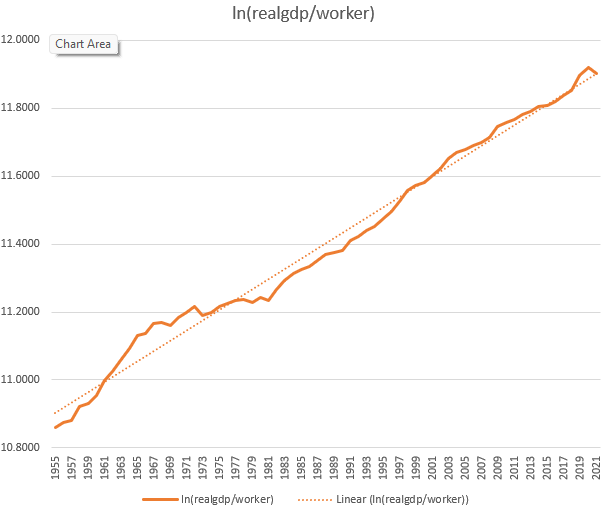
\includegraphics[width=0.6\textwidth]{graphs/lnrgdp_usa.png}
            \caption{Real GDP per Worker, US Economy
            \hyperlink{kaldor}{\beamergotobutton{Retour}}}
        \end{figure}
\end{frame}

\begin{frame}
    \frametitle{Kaldor's Stylized Facts}
    \hypertarget{capital}{} % Label for hyperlinks
    \framesubtitle{Accumulation de Capital}
        \begin{figure}
            \centering
            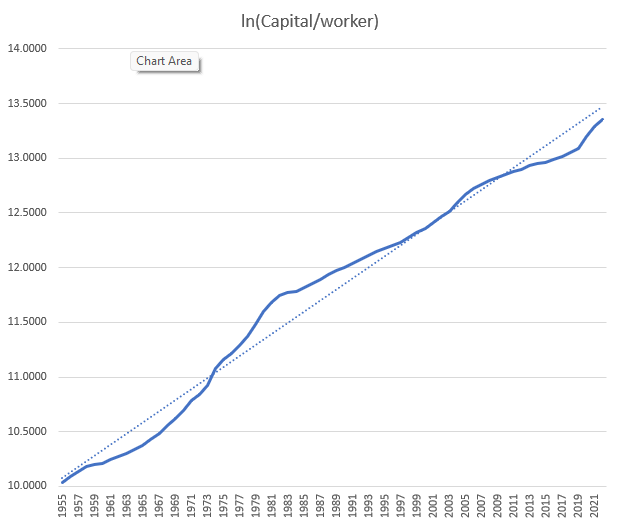
\includegraphics[width=0.6\textwidth]{graphs/lnkperworker_usa.png}
            \caption{Capital per Worker, US Economy
            \hyperlink{kaldor}{\beamergotobutton{Retour}}}
        \end{figure}
\end{frame}

\begin{frame}
    \frametitle{Kaldor's Stylized Facts}
    \hypertarget{capital_output_ratio}{} % Label for hyperlinks
    \framesubtitle{Ratio Capital-Production}
        \begin{figure}
            \centering
            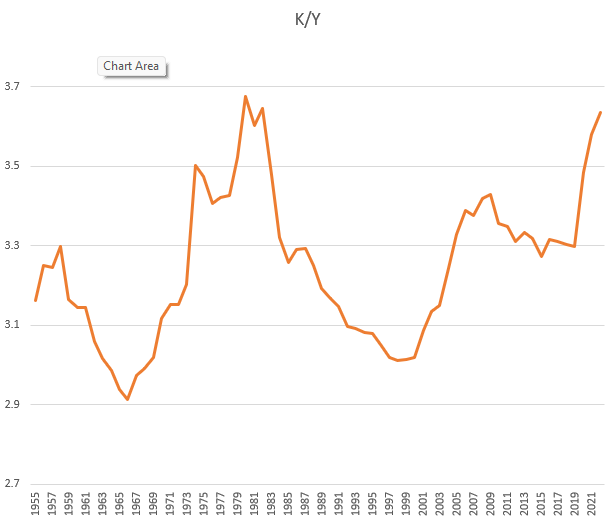
\includegraphics[width=0.55\textwidth]{graphs/kyratio_usa.png}
            \caption{\enquote*{Stability} of Capital-Output Ratio, US Economy
            \hyperlink{kaldor}{\beamergotobutton{Retour}}}
        \end{figure}
        
\end{frame}


\begin{frame}
    \frametitle{Kaldor's Stylized Facts}
    \hypertarget{income}{} % Label for hyperlinks
    \framesubtitle{Répartition du Revenu}
        \begin{figure}
            \centering
            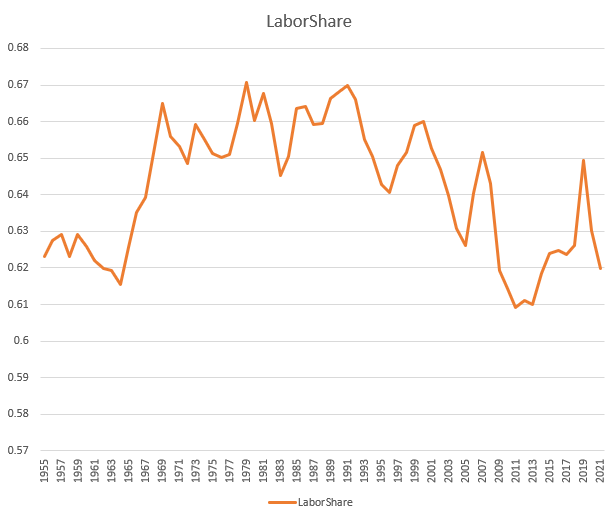
\includegraphics[width=0.6\textwidth]{graphs/labor_share.png}
            \caption{Labour Share of Income, US Economy
            \hyperlink{kaldor}{\beamergotobutton{Retour}}}
        \end{figure}
\end{frame}

\begin{frame}
    \frametitle{Kaldor's Stylized Facts}
    \hypertarget{return}{} % Label for hyperlinks
    \framesubtitle{Taux de Rendement}
        \begin{figure}
            \centering
            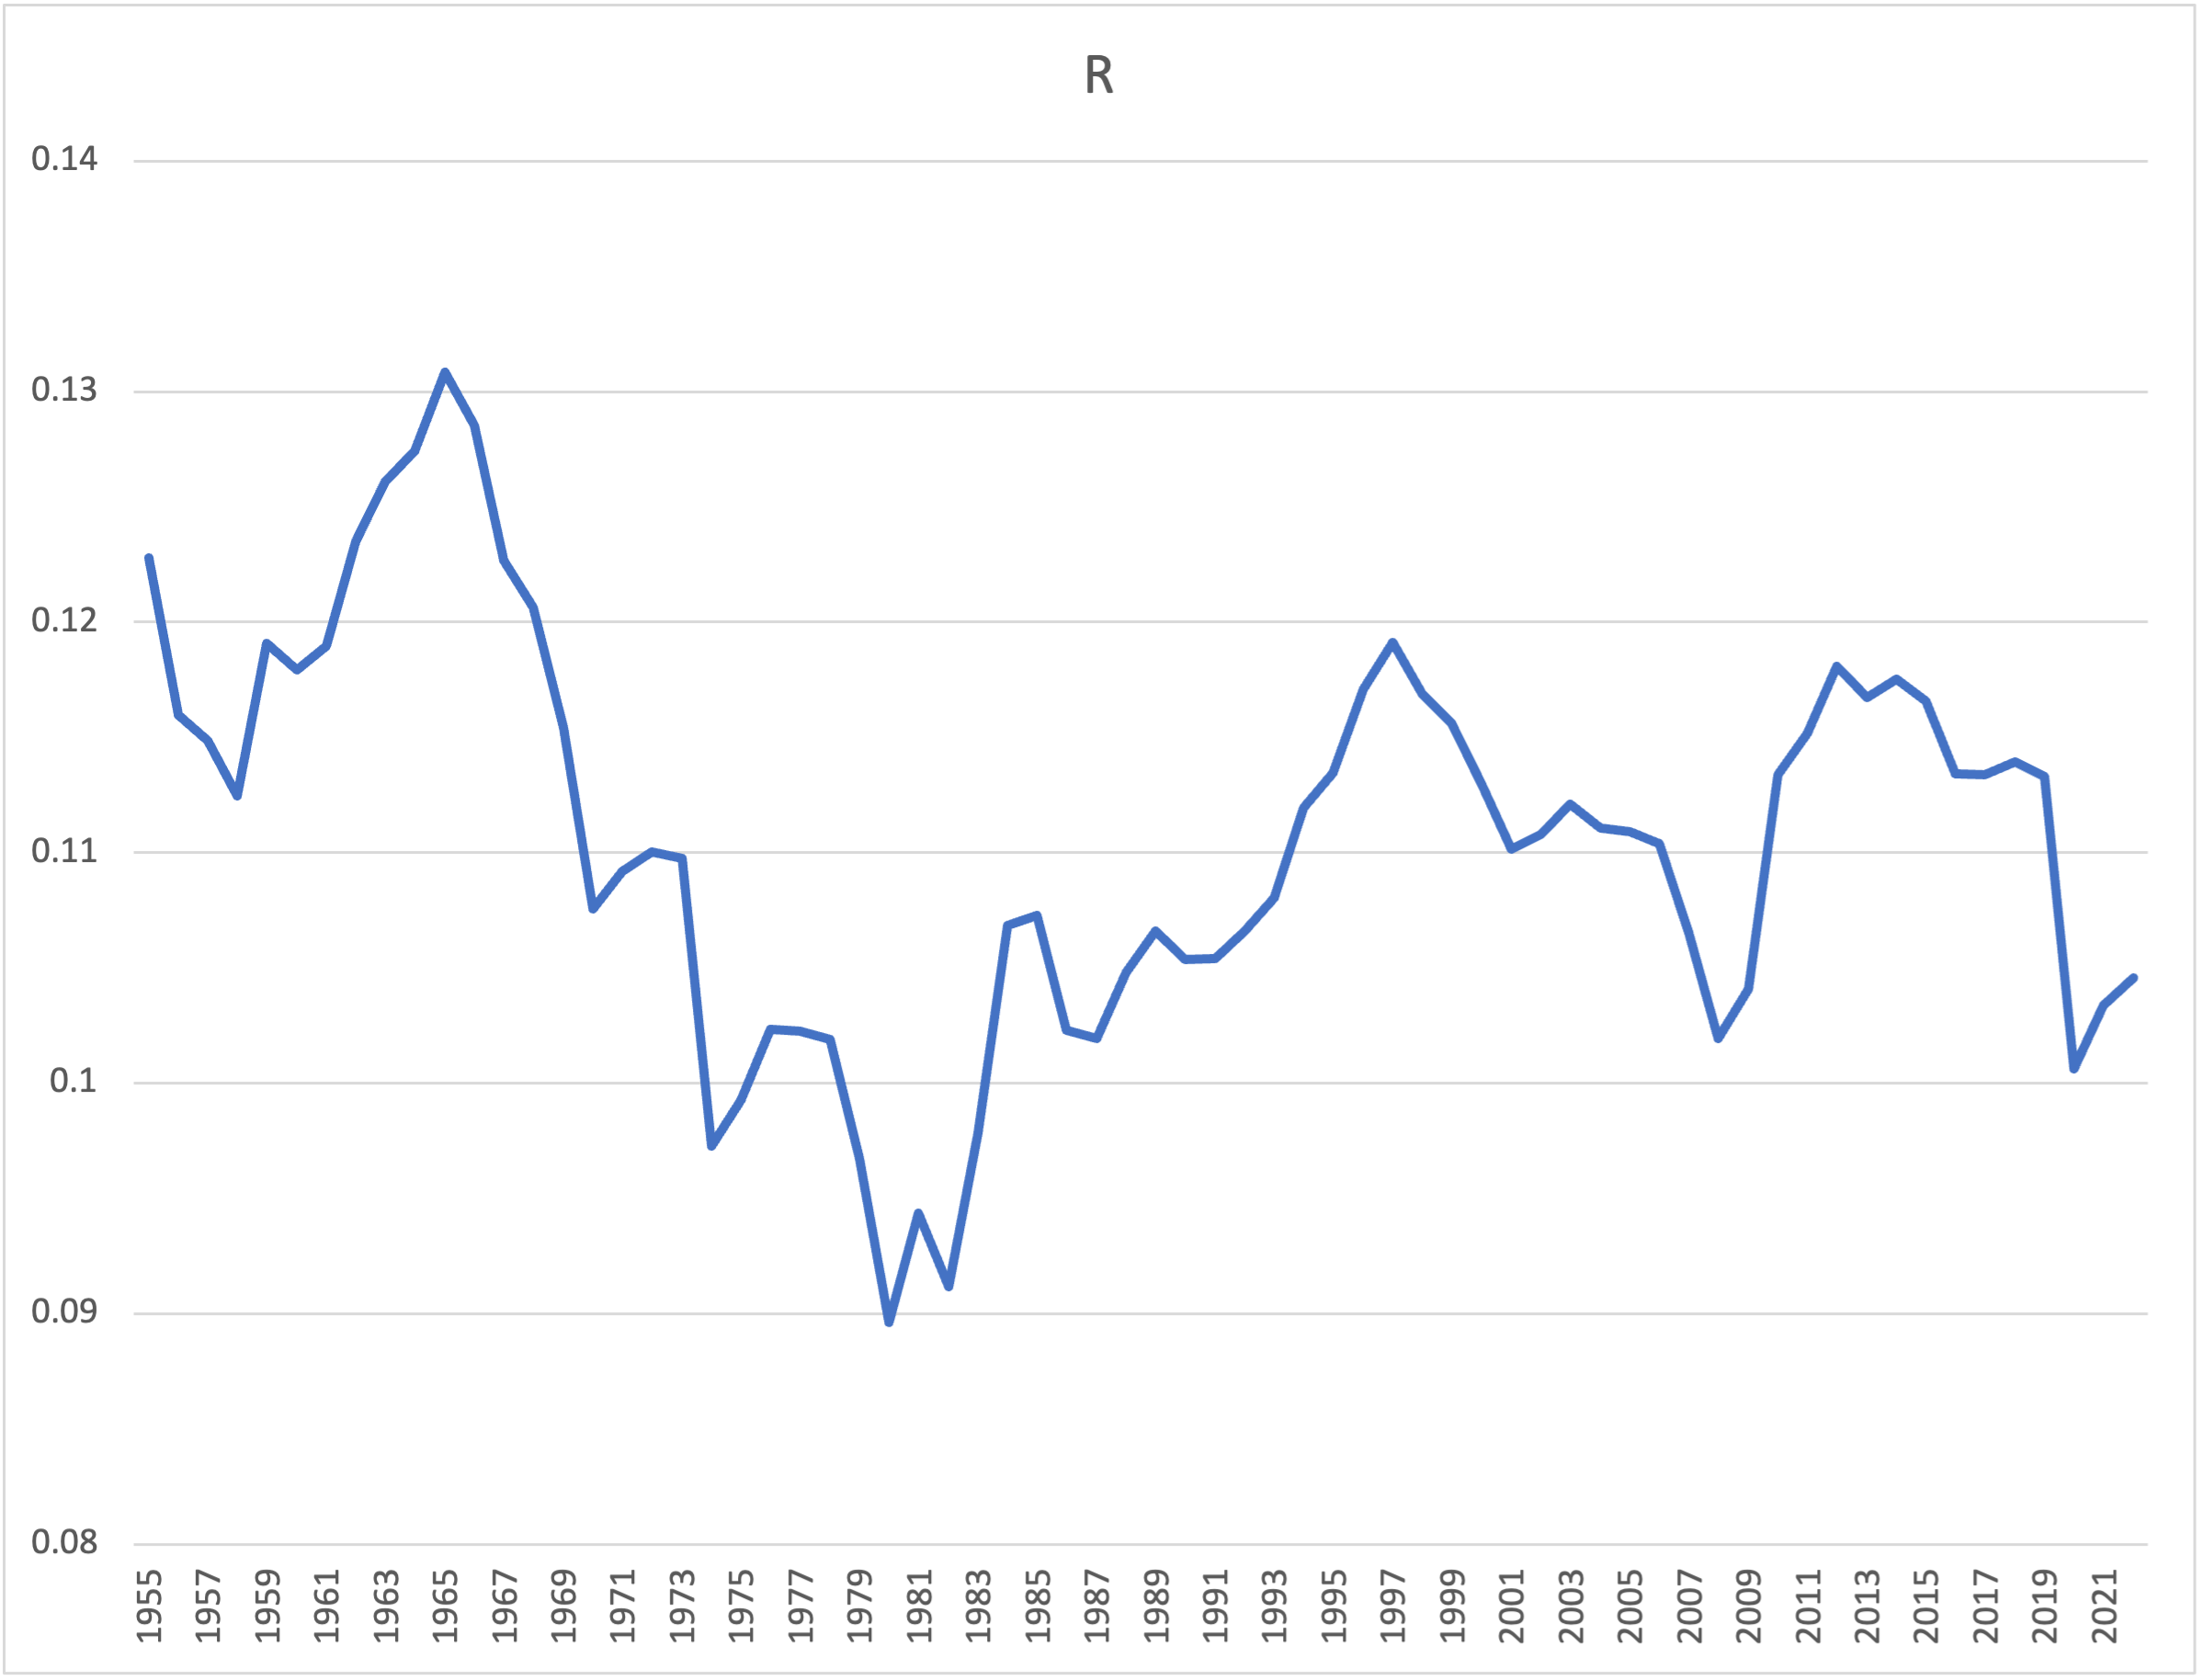
\includegraphics[width=0.6\textwidth]{graphs/r_usa.png}
            \caption{Return on Investment, US Economy
            \hyperlink{kaldor}{\beamergotobutton{Retour}}}
        \end{figure}
\end{frame}

\begin{frame}
    \frametitle{Kaldor's Stylized Facts}
    \hypertarget{wages}{} % Label for hyperlinks
    \framesubtitle{Wage Growth}
        \begin{figure}
            \centering
            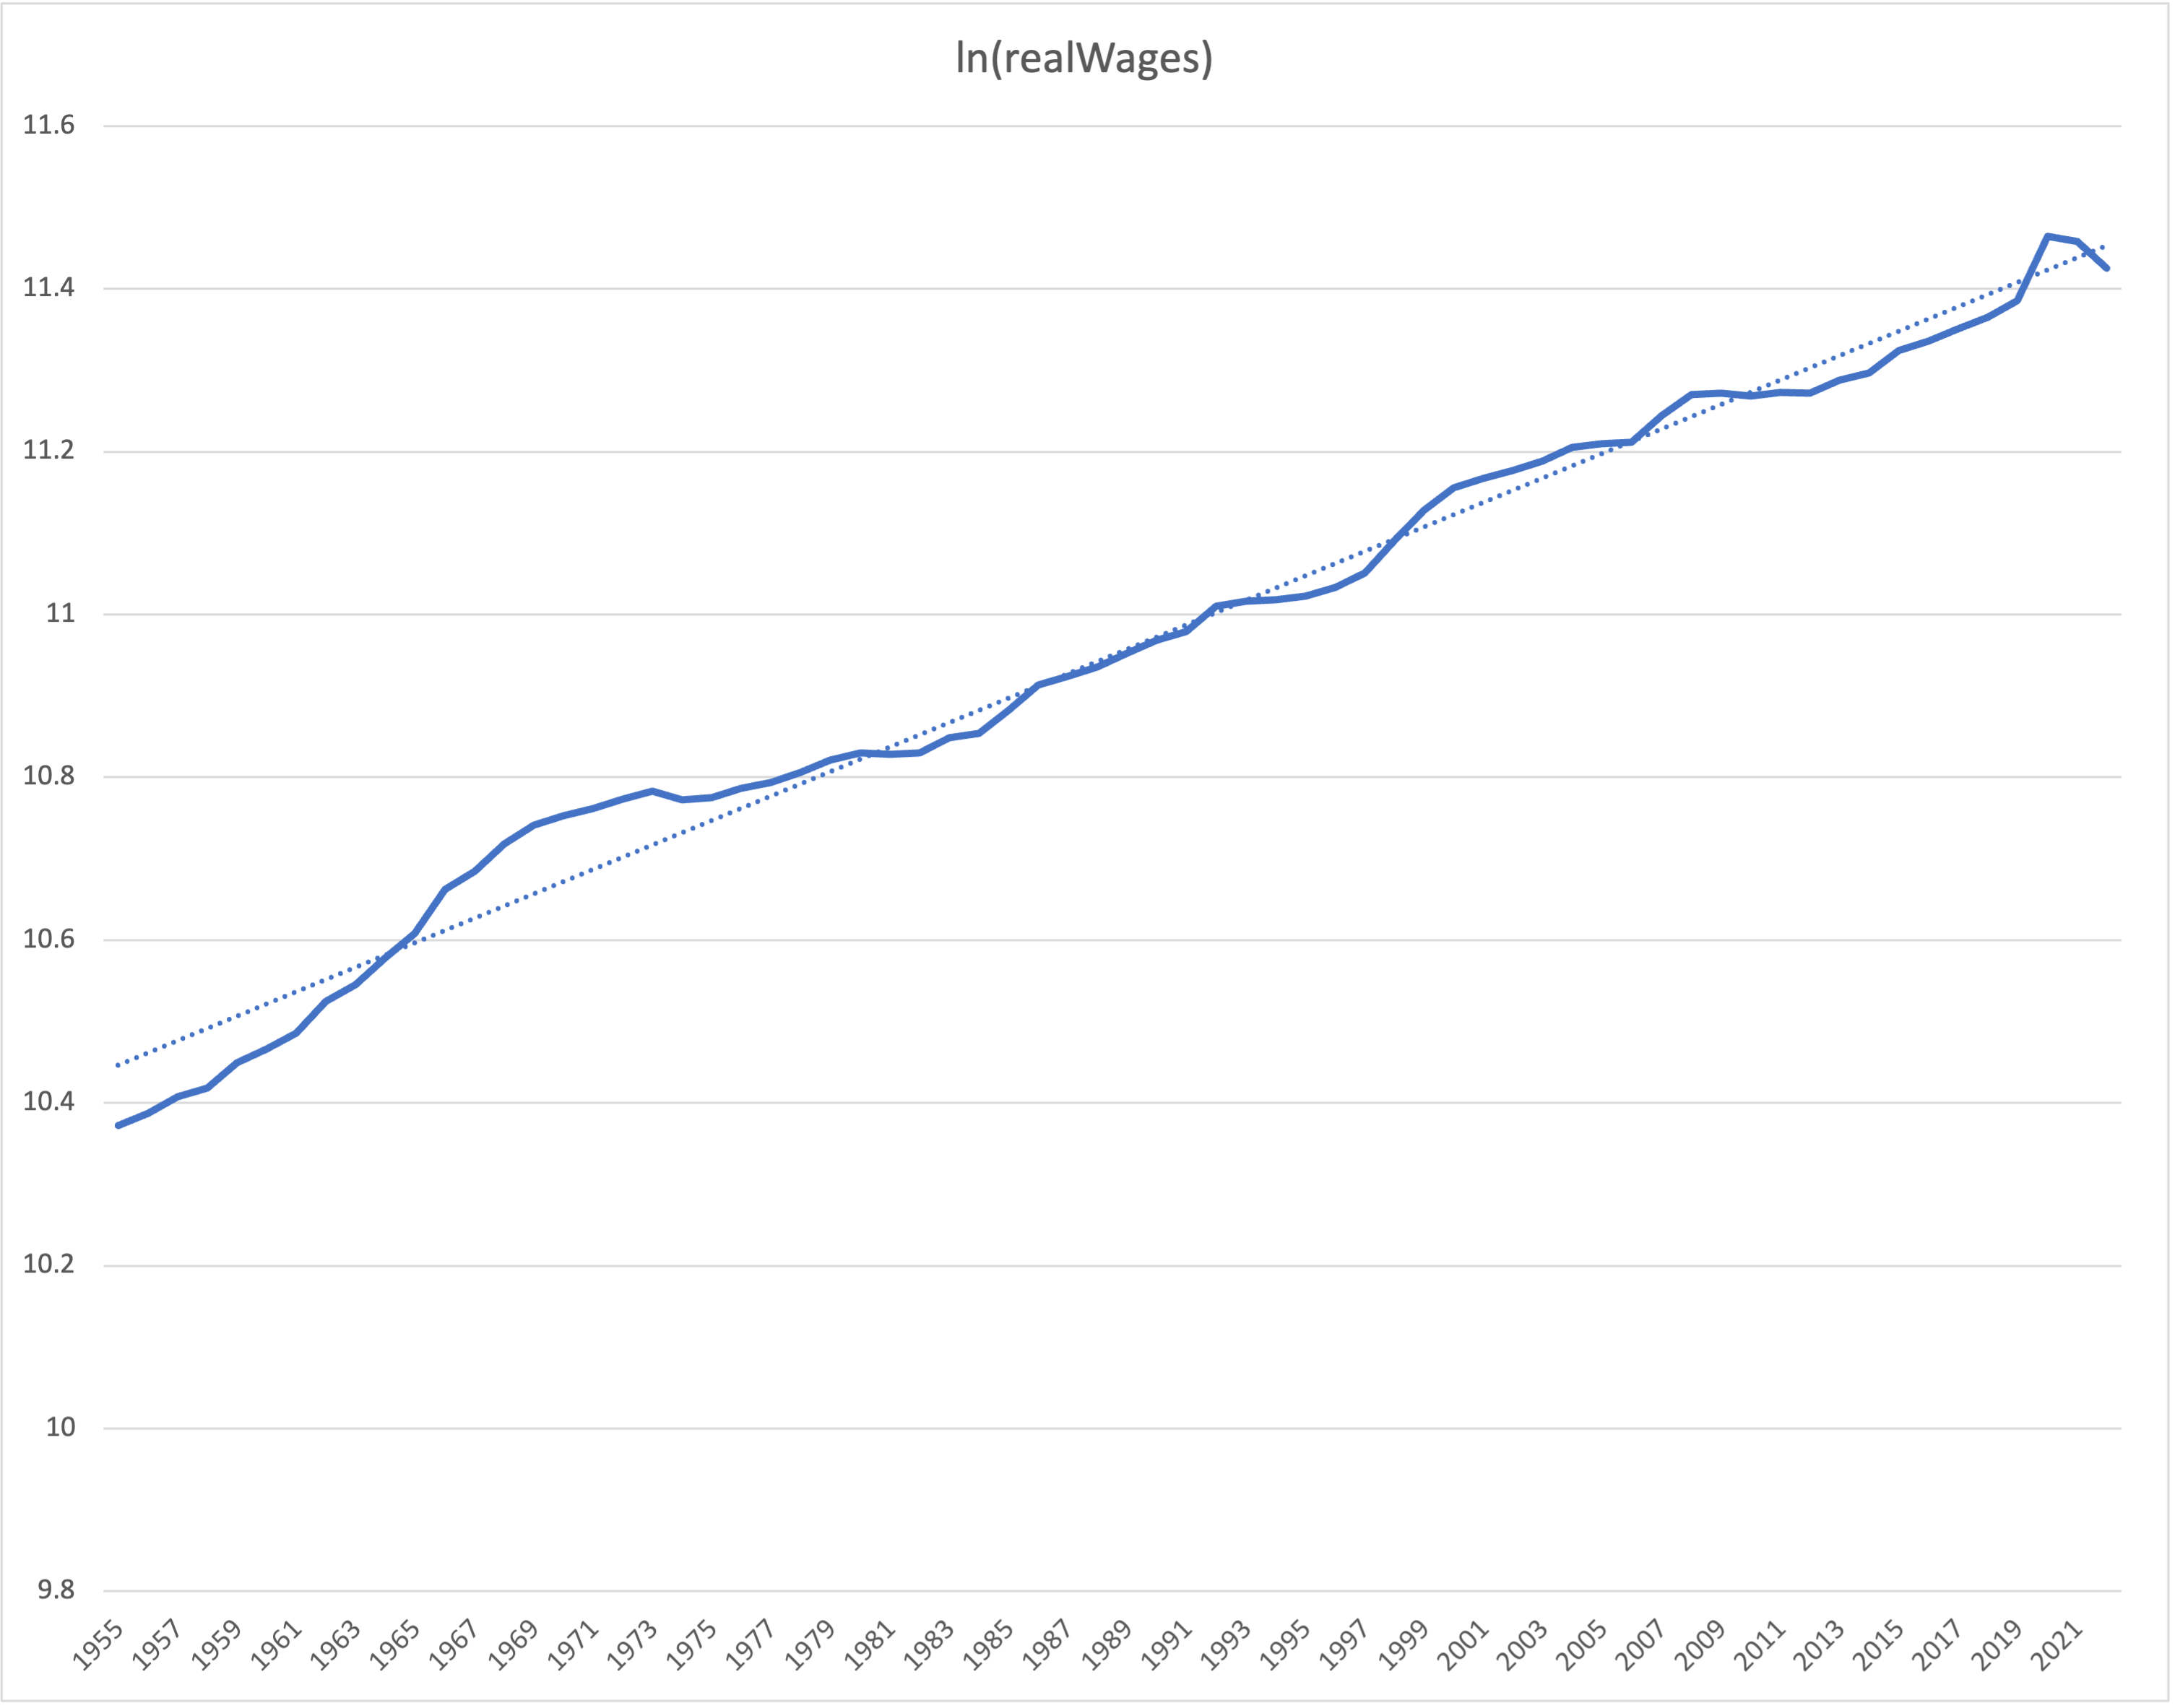
\includegraphics[width=0.6\textwidth]{graphs/lnwages_usa.png}
            \caption{Real wages, US Economy
            \hyperlink{kaldor}{\beamergotobutton{Retour}}}

        \end{figure}
\end{frame}

% \begin{frame}
%     \frametitle{Kaldor's Stylized Facts}
%     \hypertarget{return}{} % Label for hyperlinks
%     \framesubtitle{Taux de Rendement}
%         \begin{figure}
%             \centering
%             \includegraphics[width=0.8\textwidth]{graphs/}
%             \caption{Stability of Returns on Investment}
%         \end{figure}
% \end{frame}


\end{document}
